\documentclass{standalone}
\usepackage{tikz}

\usetikzlibrary{math,calc}

\begin{document}

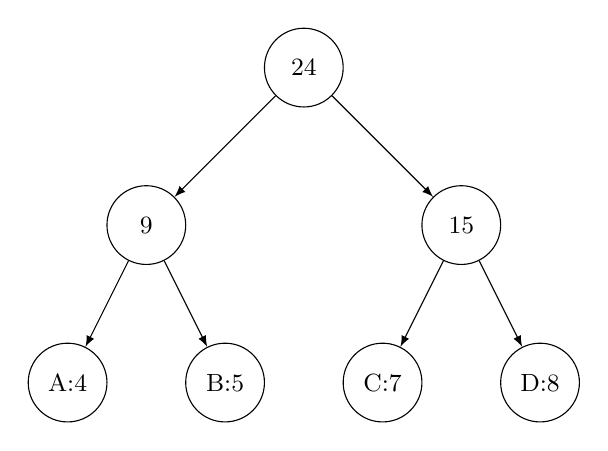
\begin{tikzpicture}[node/.style={circle,draw,minimum size=1cm,font=\small},
                    link/.style={-latex}]
  \node[node] (root) at (0,0) {24};
  \node[node] (0) at (-2,-2) {9};
  \node[node] (1) at (2,-2) {15};
  \node[node] (00) at (-3,-4) {A:4};
  \node[node] (01) at (-1,-4) {B:5};
  \node[node] (10) at (1,-4) {C:7};
  \node[node] (11) at (3,-4) {D:8};

  \foreach \from/\to in {root/0,root/1,0/00,0/01,1/10,1/11} {
    \draw[link] (\from) -- (\to);
  }
\end{tikzpicture}

\end{document}
